\section{Preguntas}

\subsection{How do you know convergence in mesh size has been achieved?}

Mesh size convergence is achieved when the solution of the problem does not change significantly with a further refinement of the mesh. This can be checked by comparing the results of the displacements, Von Mises stresses and principal stresses compared to other mesh sizes. In this case, convergence was assessed by plotting the maximum Von misses Stress with the characteristic lenght, and observing the time of processing in each case. The result shows that at an $L_c$ of 0.8, the mesh was already converging.

\begin{figure}[H]
\centering
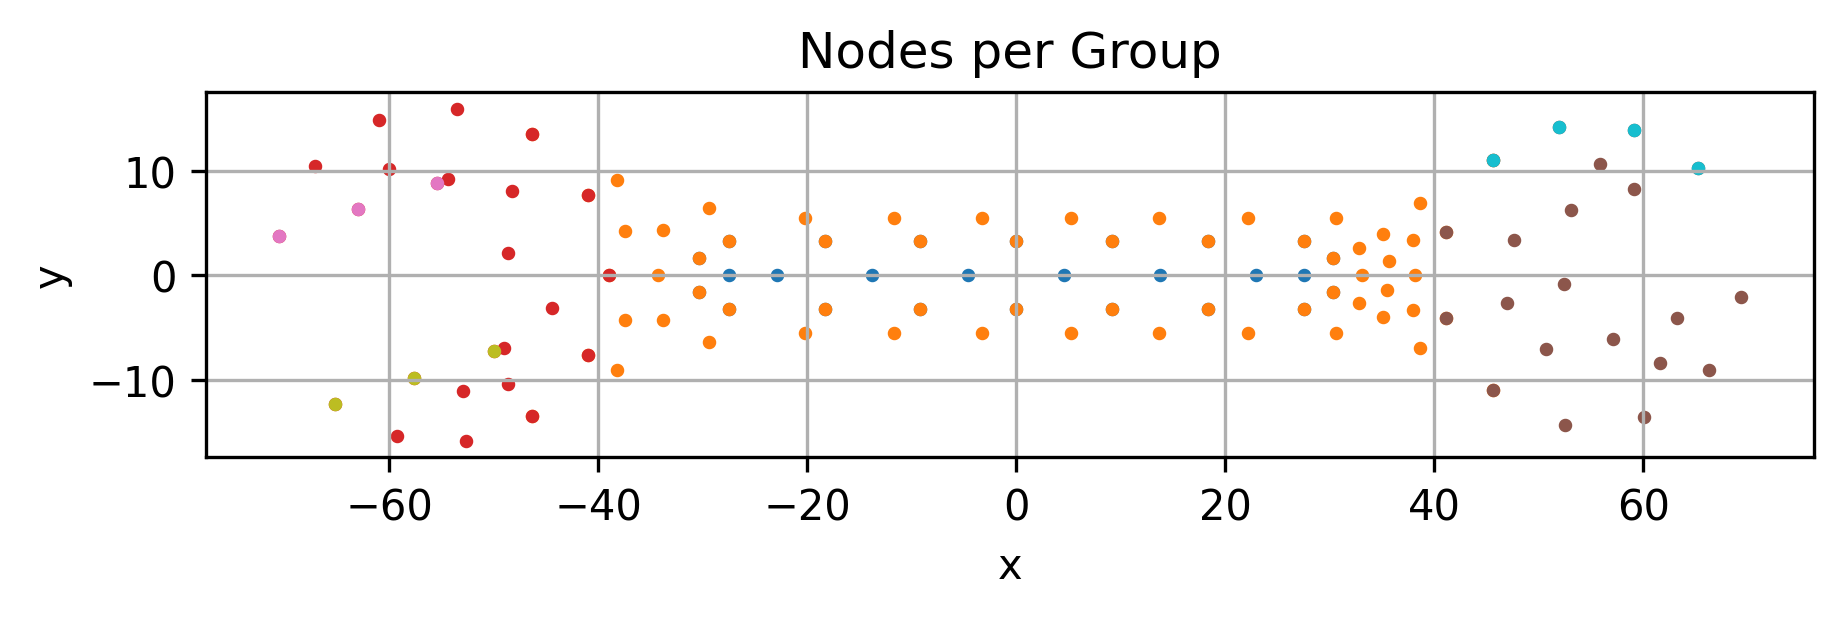
\includegraphics[width=0.5\textwidth]{GRAFICOS/Initial_nodes_por_grupo.png}
\caption{Caption}
\label{fig:wrench}
\end{figure}
  
\begin{figure}[H]
\centering
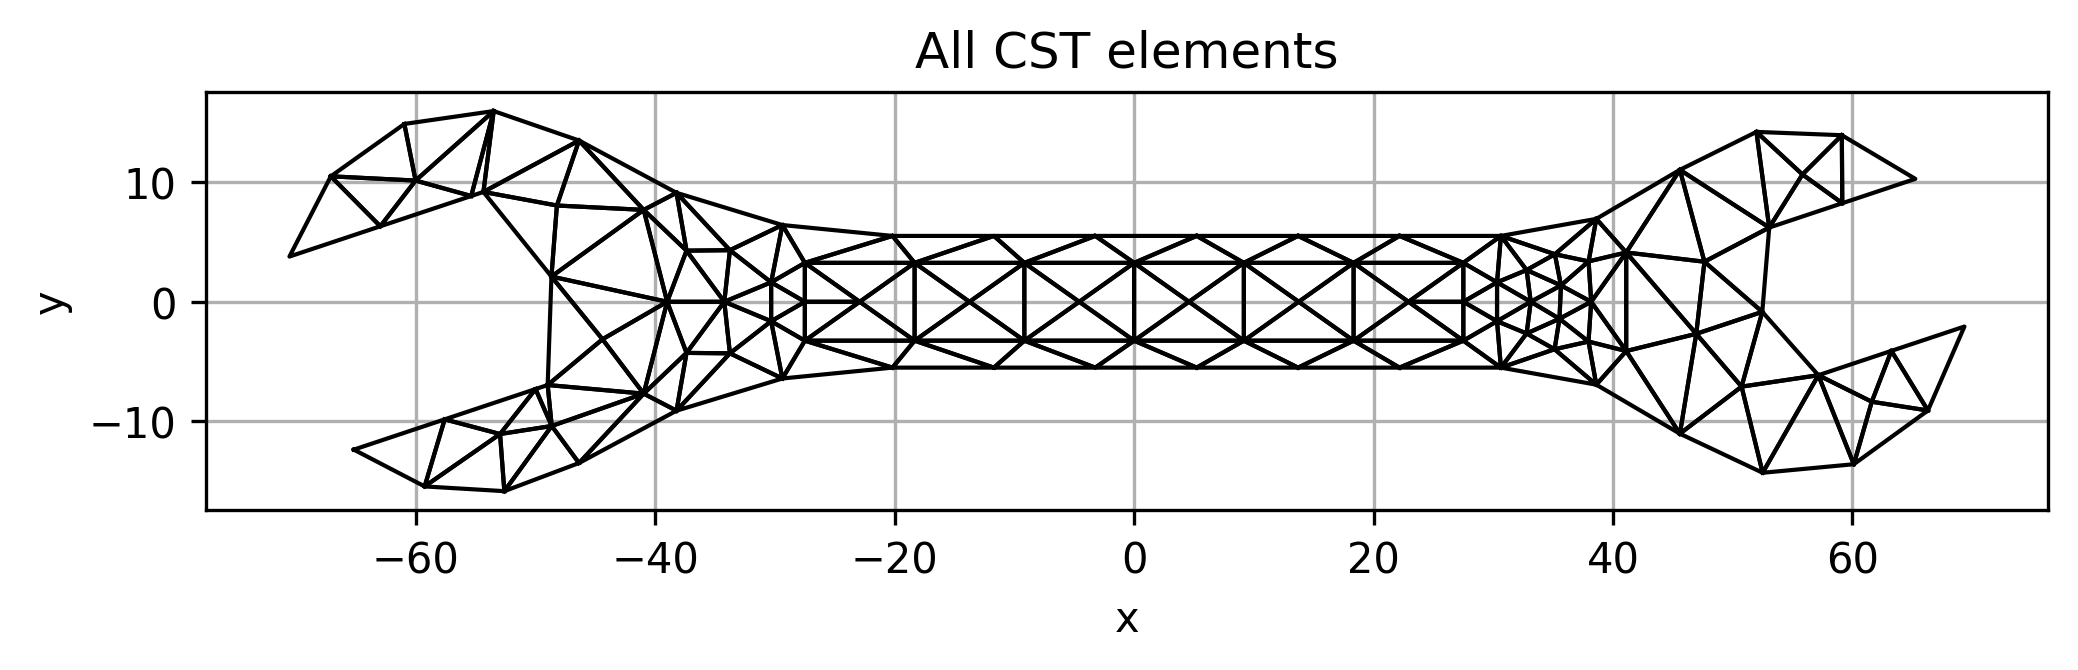
\includegraphics[width=0.5\textwidth]{GRAFICOS/Initial_elementos.png}
\caption{Caption}
\label{fig:deformed_shape}
\end{figure}
  
Then, a code was programmed to plot the convergence of the mesh depending on the time of ejecution.
  
\begin{figure}[H]
\centering
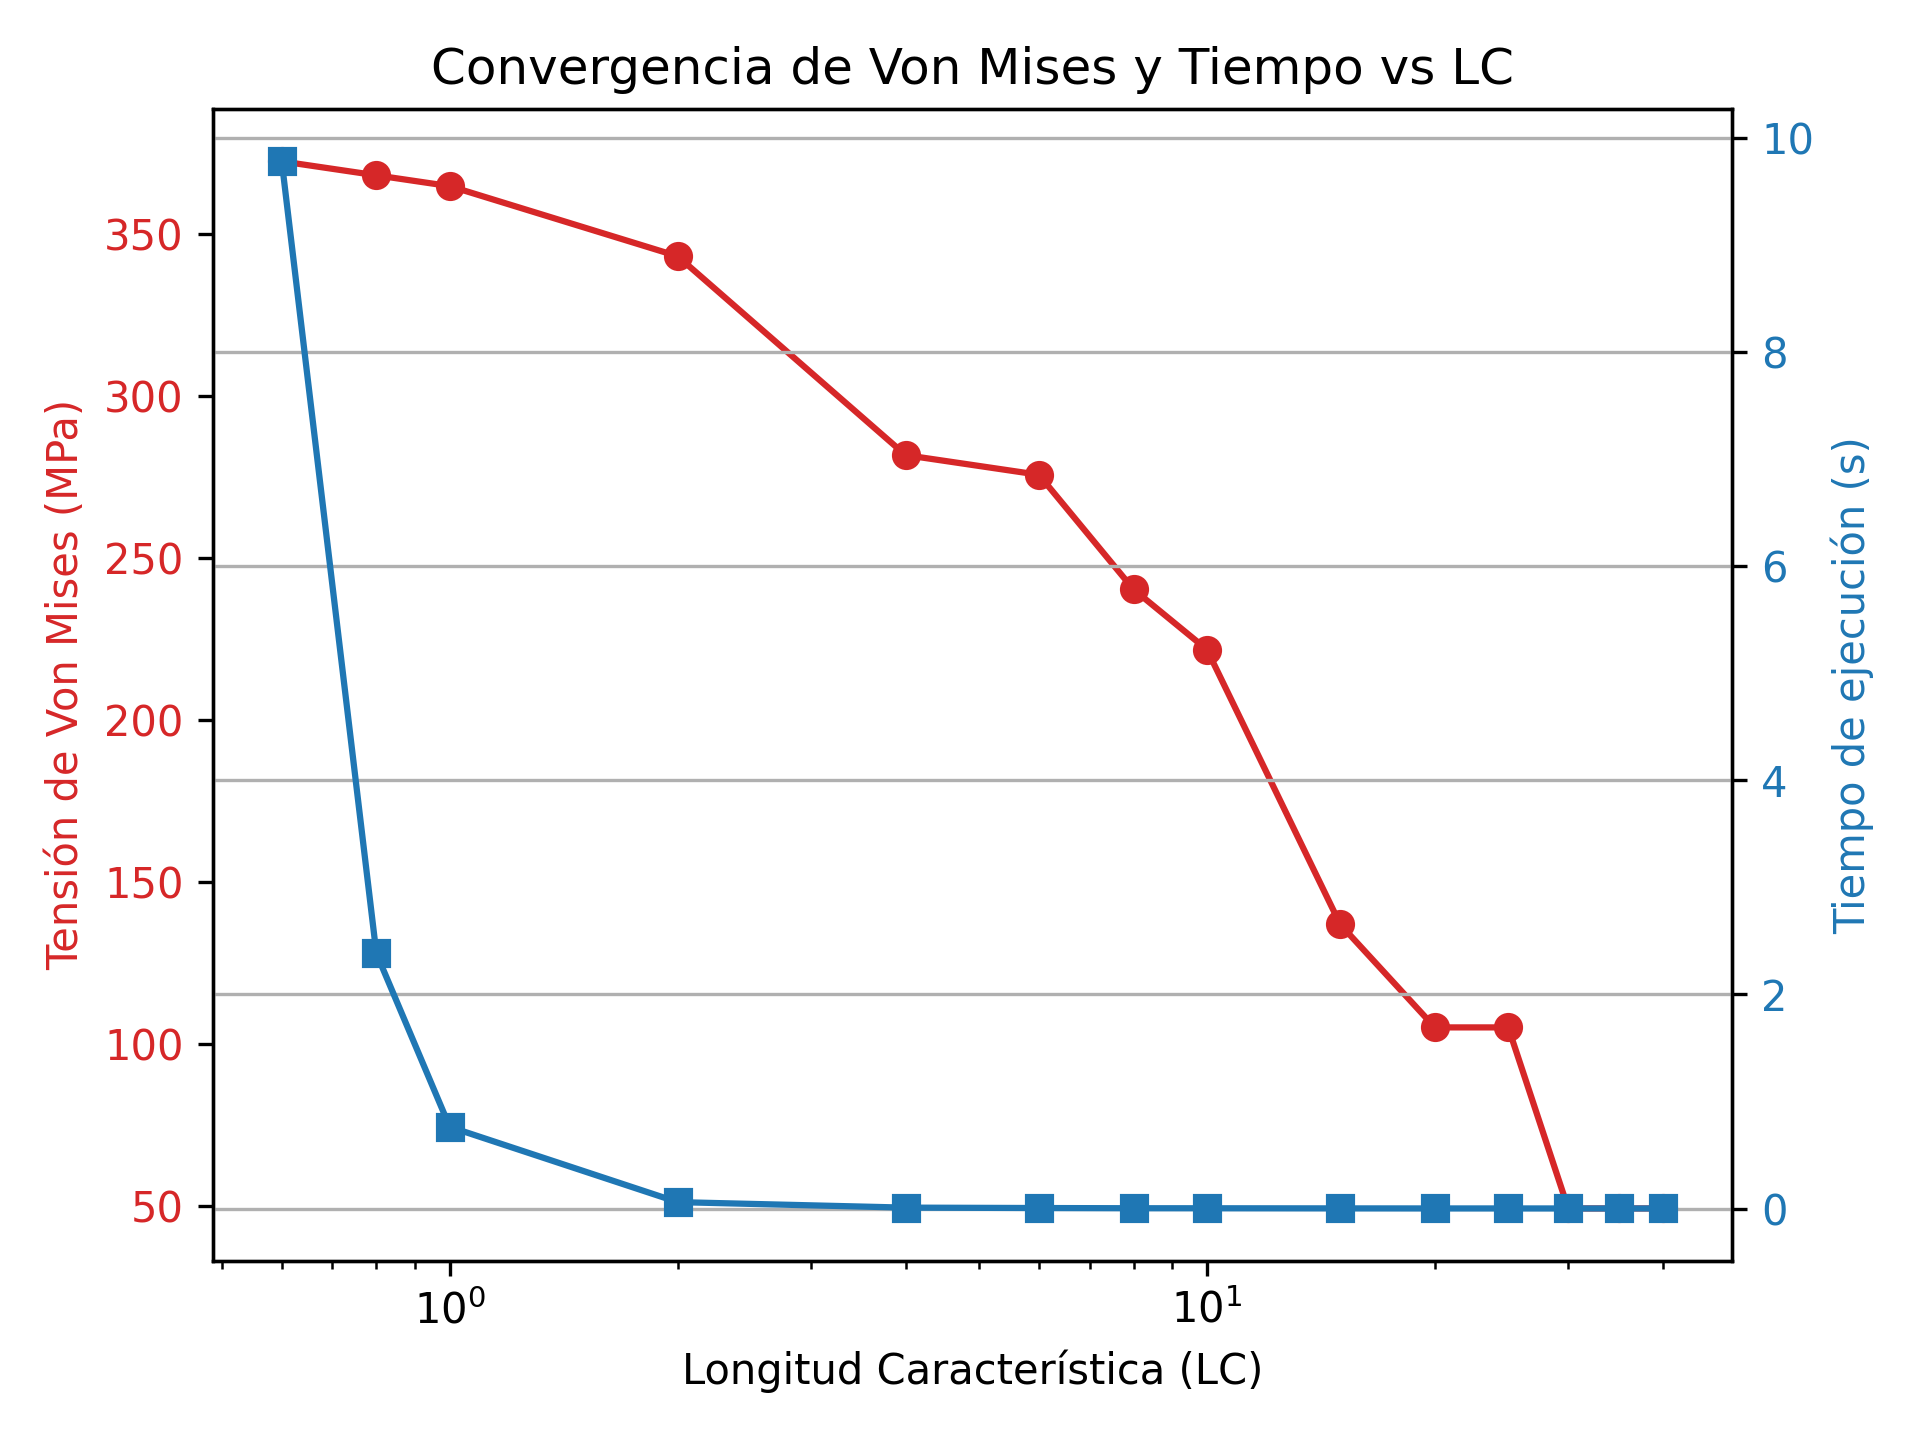
\includegraphics[width=0.6\textwidth]{GRAFICOS/convergencia.png}
\caption{Caption}
\label{fig:wrench}
\end{figure}

The result was an $L_c = 0.8$, balancing the time of computation and the precision of the model.

Therefore, the final model is plotted as follows:
  
\begin{figure}[H]
\centering
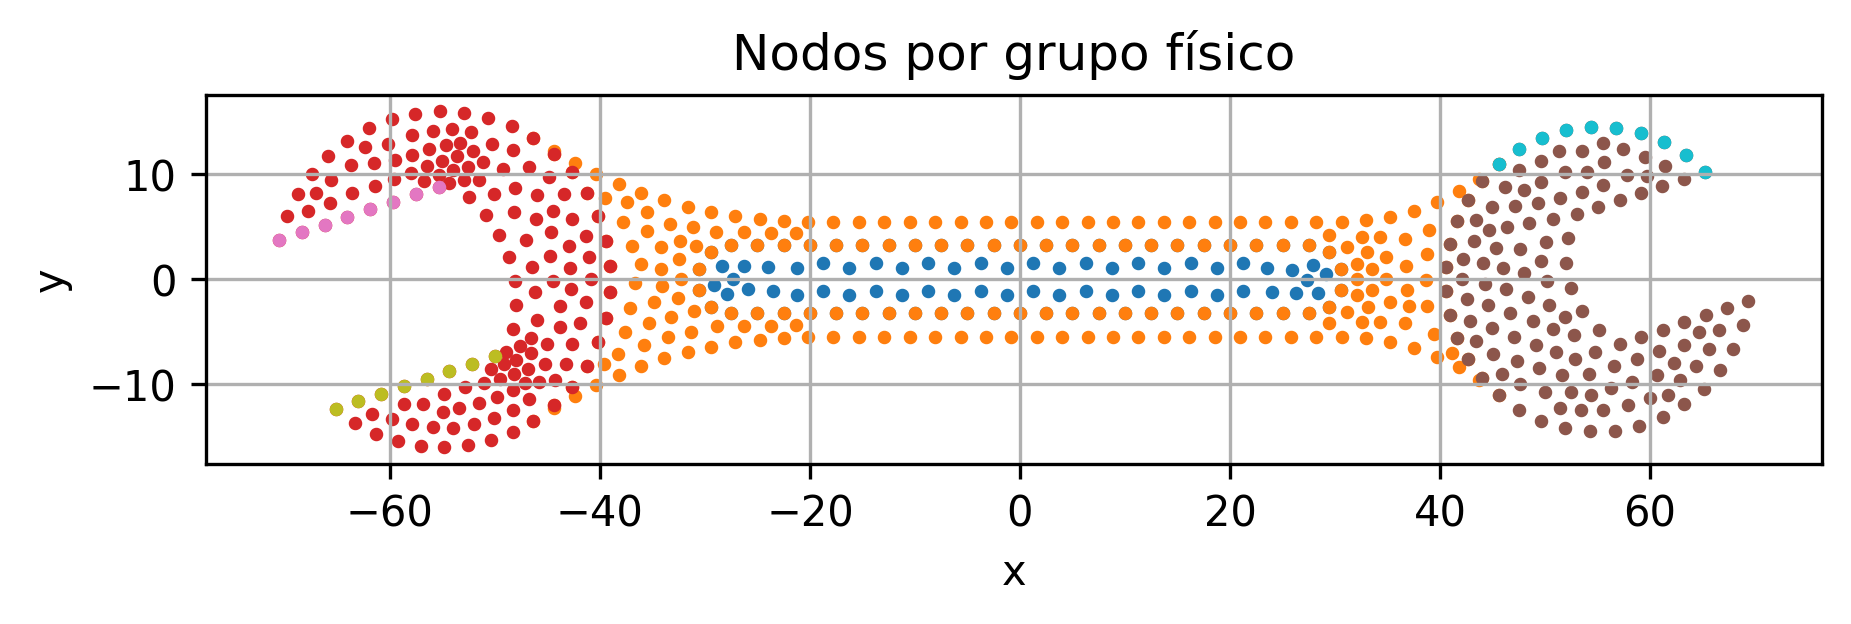
\includegraphics[width=0.5\textwidth]{GRAFICOS/Case a_nodes_por_grupo.png}
\caption{Caption}
\label{fig:wrench}
\end{figure}
  
\begin{figure}[H]
\centering
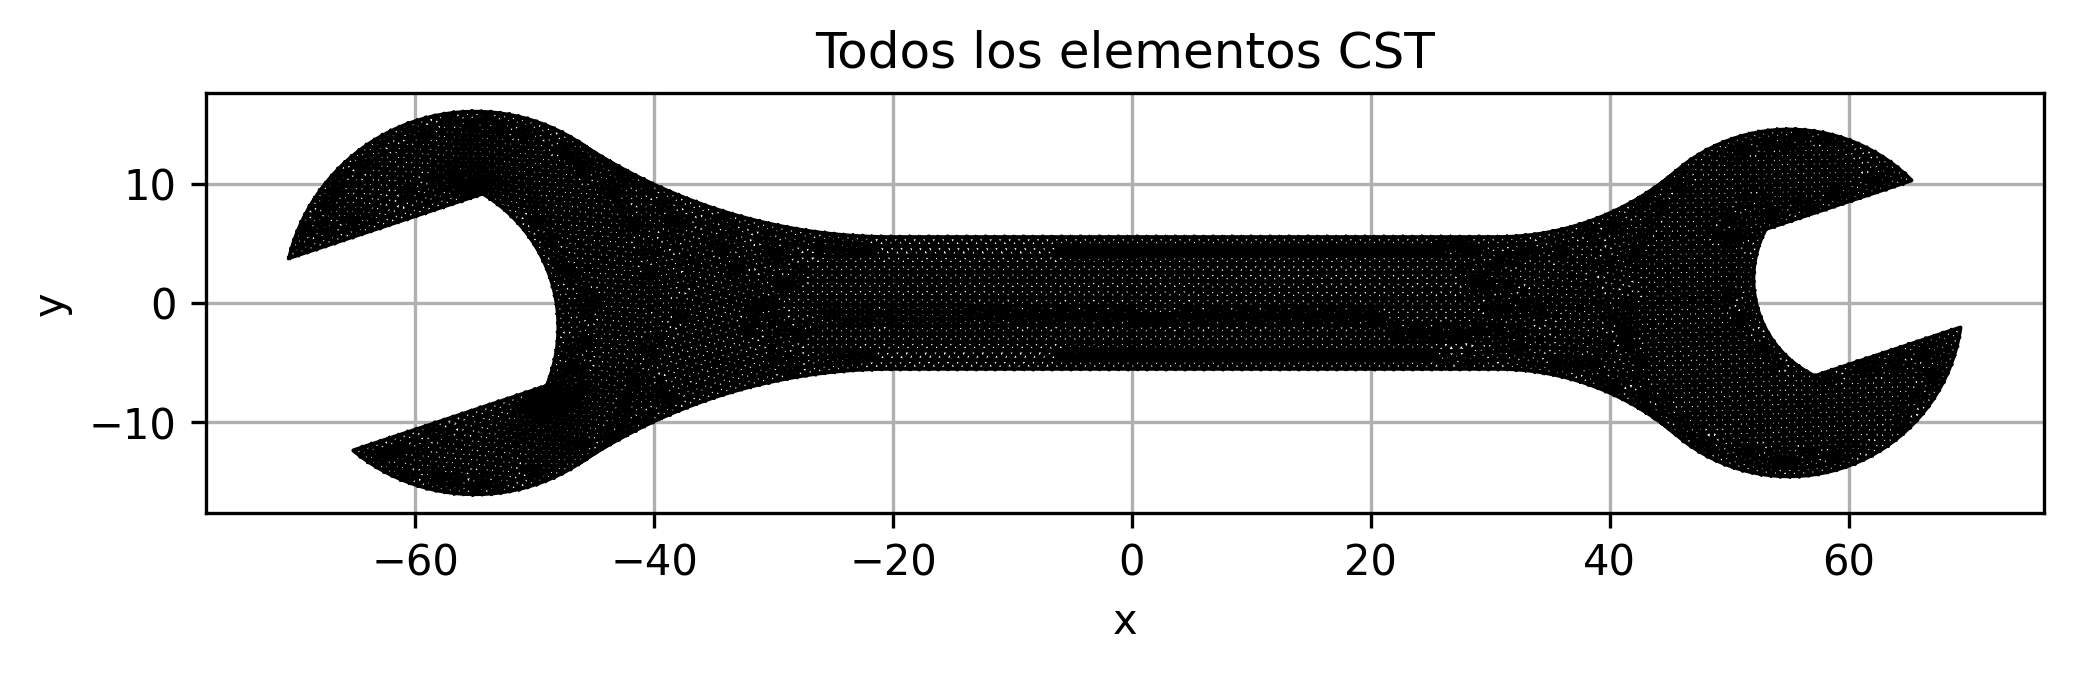
\includegraphics[width=0.5\textwidth]{GRAFICOS/Case a_elementos.png}
\caption{Caption}
\label{fig:deformed_shape}
\end{figure}

\subsection{How do the stress/strain fields look like before and after smoothing?}

Before smoothing, the stress and strain fields shows abrubt jumps between adjacent elements, producing a non-physical behaviour and dicontinuous fields. It is expected due to the implementation of CST elements, which have a constant stress and strain state. After applying post-processing smoothing, the fields becmoe continuous, whit better transitions across the domain, making it physically accurate.

\subsection{What differences do you observe when applying the load as a distributed load versus a point load?}

As a distributed load results in smoother and more realistic stress fiels, as the force is spread over an area, avoiding axcessive stress concentrations. 
On the other hand, a point load produces localized hight-stress peaks near the application point, leading to unrealistic stress values, unless the mesh is highly refined.

\subsection{Is it necessary to consider self-weight for an accurate analysis of the tool?}

In this case, it is not necessary to consider it, because the external forces applied are significantly grater than de self-weight of the PLA material. 
However, numercial comparisons showed that including self-weight, slightly increases the overall stress and displacement values, especially un ling or thin sections.

\subsection{Research or provide a reasonable stress-based failure criteria for PLA. For this loading condition, and based on
your failure criteria ¿where do you expect the wrench to fail?}

According to CITAR PAPER, PLA (Polylactic Acid) exhibits a tensile strength near 50 MPa, depending on molecular weight, crystallinity, and processing method. Additionally, the usual Young's module is about 3.5 GPa, and the material has a relatively low elongation at break (about $4\text{-}7\%$), confirming its brittle nature.

Therefore, a reasonable stress-based failure criteria for PLA under mechanical loading is the Von Mises yield criterion, assuming brittle fracture at an equivalent stress level of around 50 MPa. Given PLA's limited ductility and tendency to fail without significant plastic deformation, reaching the ultimate tensile strength would iniciate cracking or brittle rupture.

As a result, based on the FEM simulations and stress distribution results, the highest Von Mises stresses concentrated at the junction between the wrench handle and the wrench head would be an expected failure location, in other words, near sharp geometrical transitions or areas under bending moments.











